%% V1.0
%% by Shingo Mori

\documentclass[10pt,journal,compsoc]{IEEEtran}

\usepackage[pdftex]{graphicx}    
\usepackage{cite}
\usepackage{subfig}
\hyphenation{op-tical net-works semi-conduc-tor}


\begin{document}

\title{Map My World Writeup}

\author{Shingo Mori}

\markboth{SLAM project, Robotics Nanodegree Program, Udacity}%
{}
\IEEEtitleabstractindextext{%

\begin{abstract}
The goal of this project is to create a ROS package that utilizes RTAB-Map to solve SLAM problem in a gazebo environment. A manually controlled robot moves around in the environment while the algorithm attempts to create a map in real-time using sensor data acquired by the robot. SLAM is tested in two different environments. The package successfully maps the both environments.
\end{abstract}

% Note that keywords are not normally used for peerreview papers.
\begin{IEEEkeywords}
Udacity, SLAM, ROS, RTAB-Map.
\end{IEEEkeywords}}


\maketitle
\IEEEdisplaynontitleabstractindextext
\IEEEpeerreviewmaketitle
\section{Introduction}
\label{sec:introduction}

\IEEEPARstart{S}{imultaneous} Localization and Mapping (SLAM) problem is one of the most fundamental problems in robotics. The SLAM problem arises when a robot does not have access to the map of an environment, nor does it know its own pose. SLAM is especially important for indoor mapping, where external measurements like GPS are unavailable and the robot poses must be inferred using only internal measurement and control data.

The goal of this project is to create a ROS package that is able to solve the SLAM problem in a simulated environment.

\section{Background}
There are many algorithms exist to solve the SLAM problem. Several approaches are discussed in the Probabilistic Robotics book \cite{Thrun:2005:PR:1121596}, including the extended Kalman Filter SLAM (EKF SLAM), the Fast SLAM and the Graph SLAM.

The EKF SLAM is one of the earliest solution for the SLAM problem. It takes discrete features and controls as input and makes a Gaussian noise assumption to estimate the robot pose. It is easy to implement, but suffers from a quadratic cost as the number of features grow and only works for the noises that follow a unimodal Gaussian distribution.

\subsection{Fast SLAM}
The Fast SLAM applies the Monte Carlo Localization algorithm where particles are used to represent the posterior hypotheses. Each feature locations are estimated individually using low-dimensional Gaussian distribution. This allows the algorithm to run in time logarithmic in the number of features. Additionally, because data associations are made on each particle, the algorithm is robust to non-linear data association problems. Although the algorithm is formulated to calculate the full path posterior, since particle filters are updated incrementally, the algorithm can also estimate momentary robot poses.

The original Fast SLAM is landmark-based. Hence it cannot model arbitrary environments. However, the Grid-based Fast SLAM algorithm overcomes this problem by applying the Fast SLAM to Occupancy Grid Map. There is an implementation of Grid-based Fast SLAM in the official ROS package called gmapping.

\subsection{Graph SLAM}
The Graph SLAM estimates full posteriors over all poses and features of the map. The algorithm creates a sparse graph composed of motion and measurement constraints. By optimizing those constraints, a maximum likelihood of robot poses is estimated. This graph optimization technique enables the algorithm to utilize full data to improve data association problem.

The algorithm initializes its graph by adding all the non-linear constraints. Then the full posterior is inferred by iteratively linearizing the constraints using the Taylor Series and solving the equation. The estimated pose vector gets better on each iteration, and should converge after a certain number of iterations.

\subsection{RTAB-Map}
RTAB-Map (Real-Time Appearance-Based Mapping) is a Graph-Based SLAM algorithm implemented in the official ROS package. It subscribes to RGB-D sensor data and optionally to laser data and odometry data. It publishes the estimated map in several ways including the Occupancy Grid Map.

The algorithm has three main characteristics. An incremental appearance-based loop closure detector \cite{labbe14online}, an efficient memory management, and an Front-end and Back-end structure. An overview image of the process created by M. Labbé \cite{Labbe:2015:IntRoLab:RTABMap} is shown in Fig. \ref{fig:rtabmap-overview}.

\begin{figure}[thpb]
      \centering
      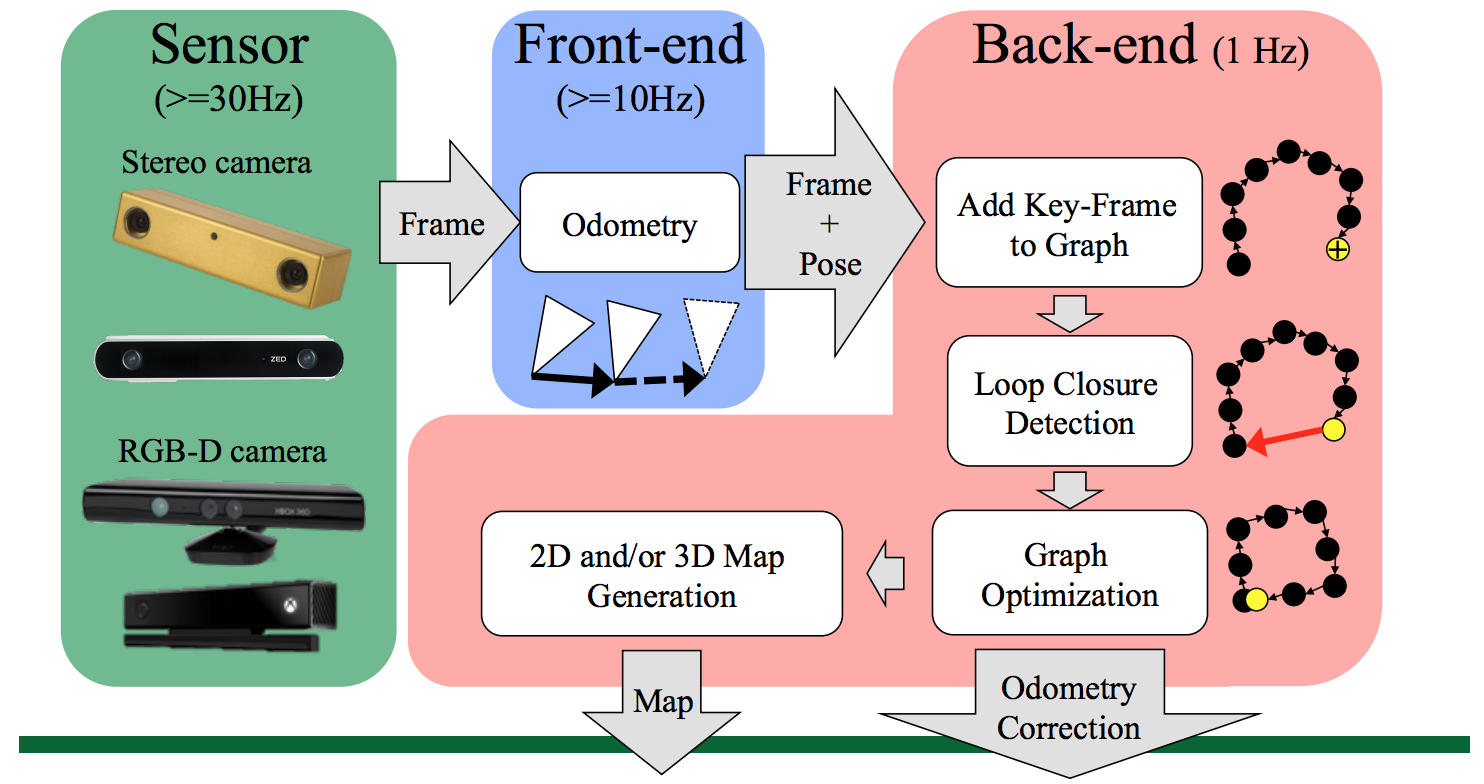
\includegraphics[width=0.9\linewidth]{rtabmap-overview}
      \caption{Overview of the RTAB-Map algorithm.}
      \label{fig:rtabmap-overview}
\end{figure}

\subsection{Comparison}
There are two major forms of the SLAM problem, the online SLAM and the full SLAM. The former involves estimating the most recent pose of the robot, whereas the latter seeks to estimate the full posterior over the entire path.

Although the Fast SLAM approach and its implementations are able to solve the full SLAM problem, it is more suited to solving the online SLAM problem. Graph-based SLAM, on the other hand, is better suited for solving the full SLAM problem due to its graph-optimization approach. 

RTAB-Map, a Grid-based algorithm, is used since we aim to create a map as accurate as possible in this project.

\section{Scene and robot configuration}
A robot is generated and manually navigated in a gazebo environment. A ROS package is created to subscribe to the sensor data attached to the robot, and to publishe the estimated map of the environment using RTAB-Map.

\subsection{Environments}
The package is tested in two different environments. Images of the first environment, Kitchen Dining, is shown in Fig. \ref{fig:supplied-image}. This environment is supplied by Udacity. Images of the second environment, Bot Cafe, is shown in Fig. \ref{fig:personal-image}. This environment is created using the Gazebo Building Editor.

\begin{figure}[thpb]
      \centering
      \subfloat[Overview]{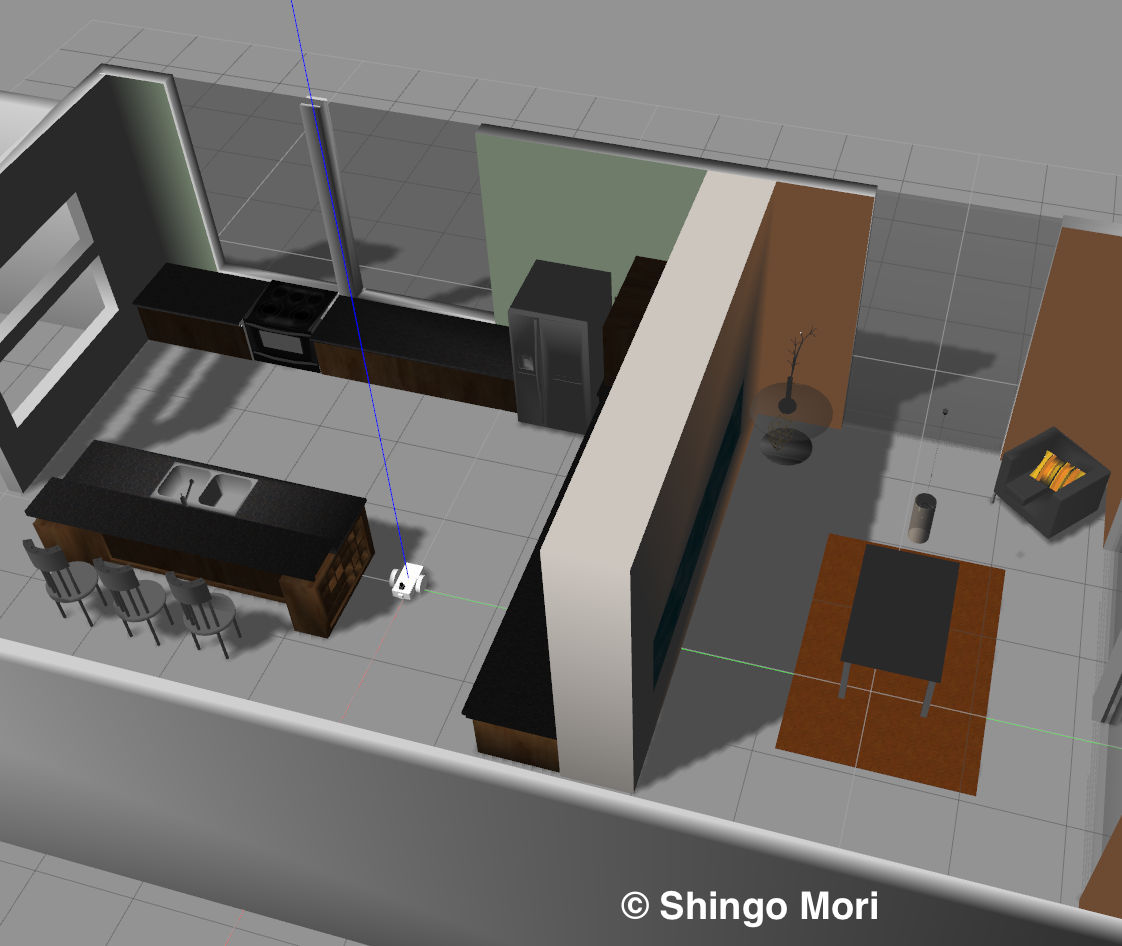
\includegraphics[width=0.8\linewidth]{supplied-overview}}
      \vfill
      \subfloat[Top View]{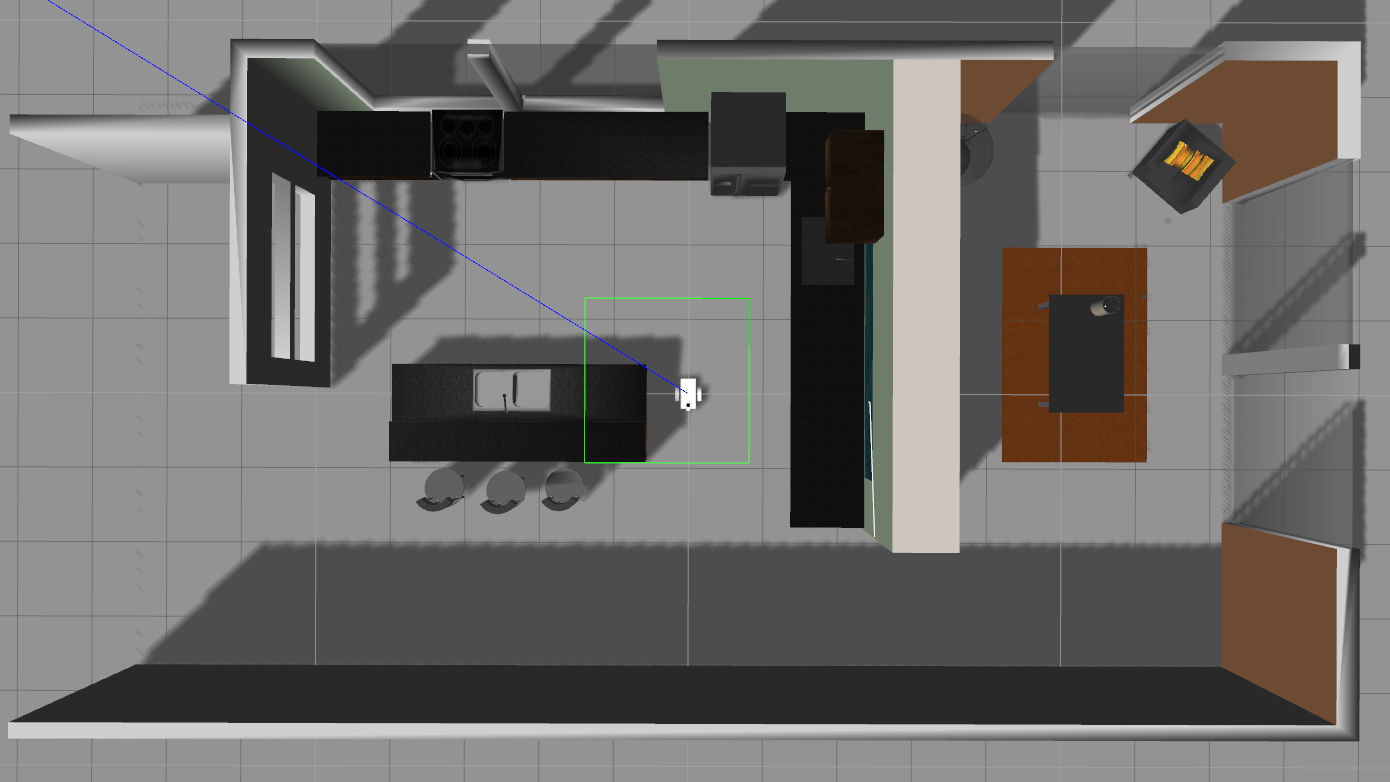
\includegraphics[width=0.8\linewidth]{supplied-top}}
      \caption{Image of the Kitchen Dining environment.}
      \label{fig:supplied-image}
\end{figure}

\begin{figure}[thpb]
      \centering
      \subfloat[Overview]{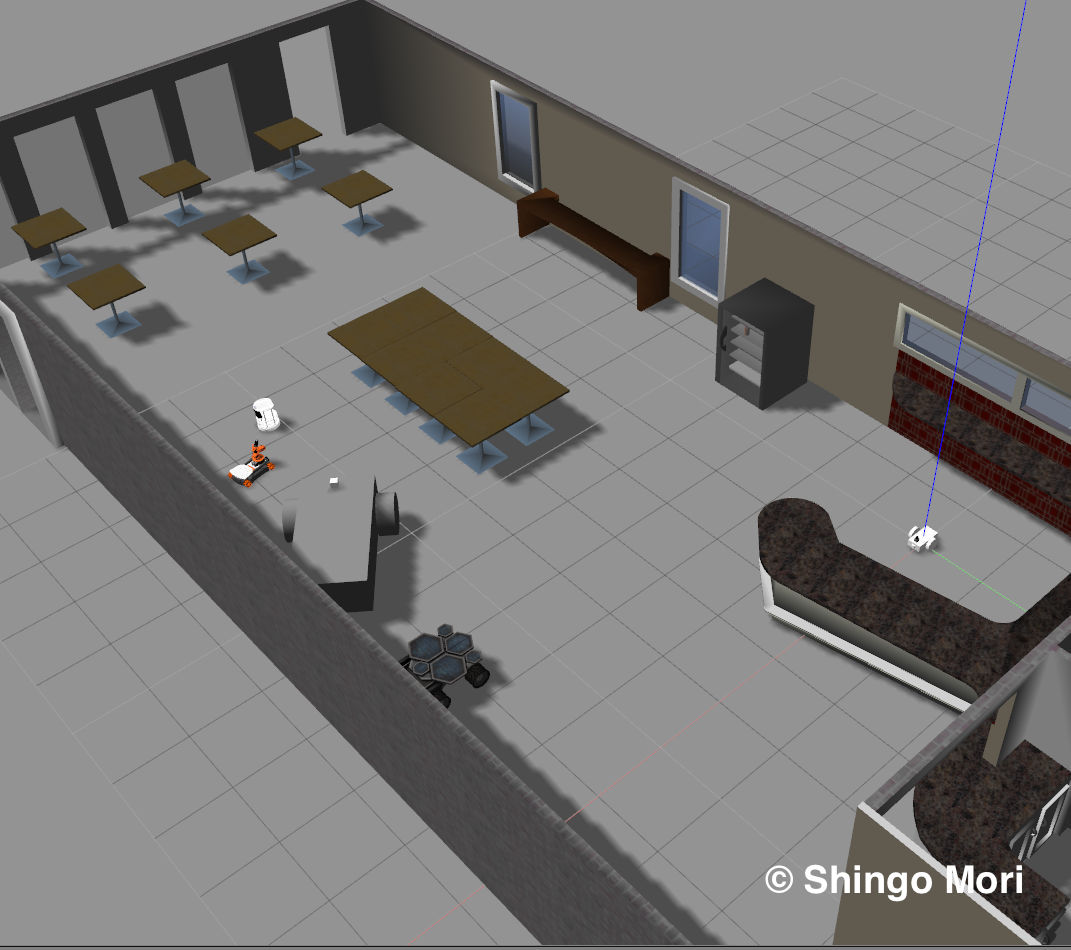
\includegraphics[width=0.8\linewidth]{personal-overview}}
      \vfill
      \subfloat[Top view]{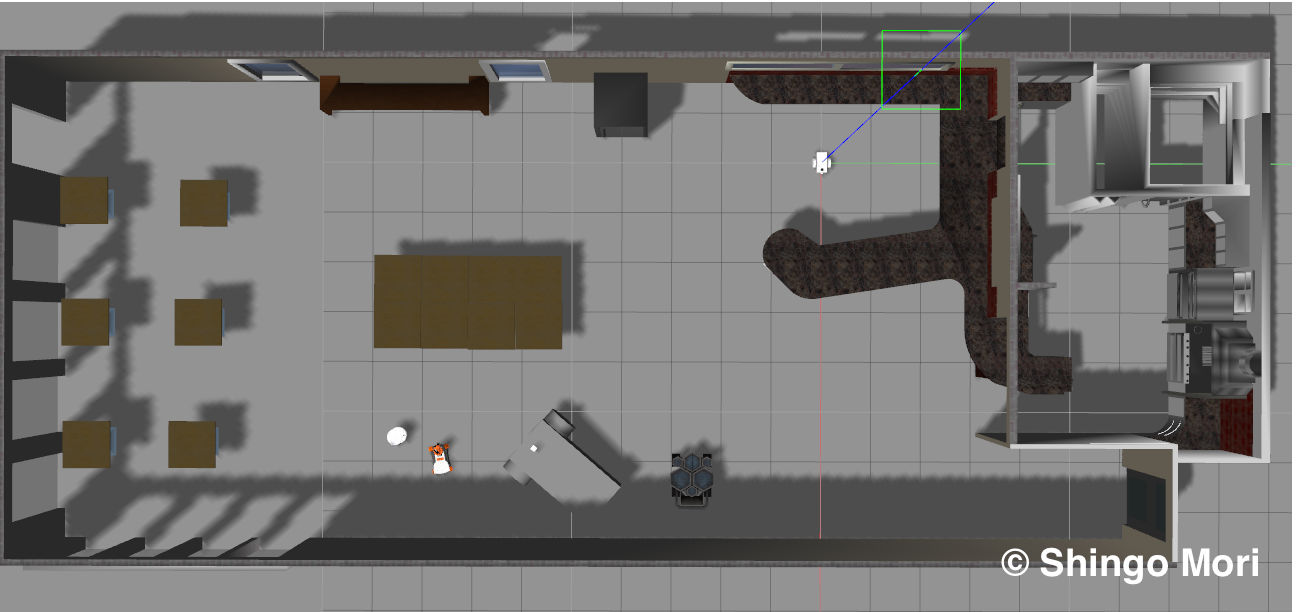
\includegraphics[width=0.8\linewidth]{personal-top}}
      \caption{Image of the Bot Cafe environment.}
      \label{fig:personal-image}
\end{figure}

\subsection{Model design}
The robot used in this project is a differential wheeled robot attached with a RGB-D camera, a laser range finder, and a wheel odometry sensor. An image of the robot model is shown in Fig. \ref{fig:robot-model}, and the graph of the tf-coordinates is shown in Fig. \ref{fig:tf-view}.

\begin{figure}[thpb]
      \centering
      \subfloat[Robot model]{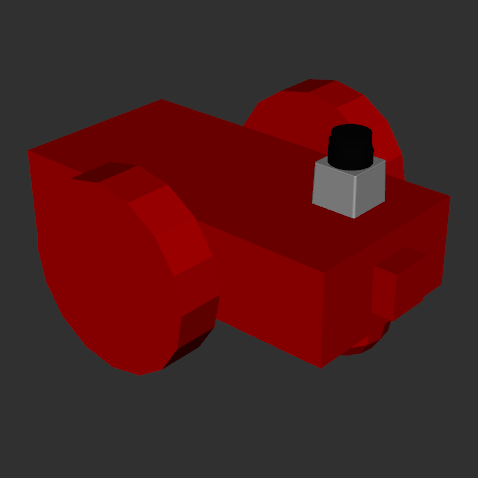
\includegraphics[width=0.32\linewidth]{robot-model}\label{fig:robot-model}}
      \hfill
      \subfloat[tf graph]{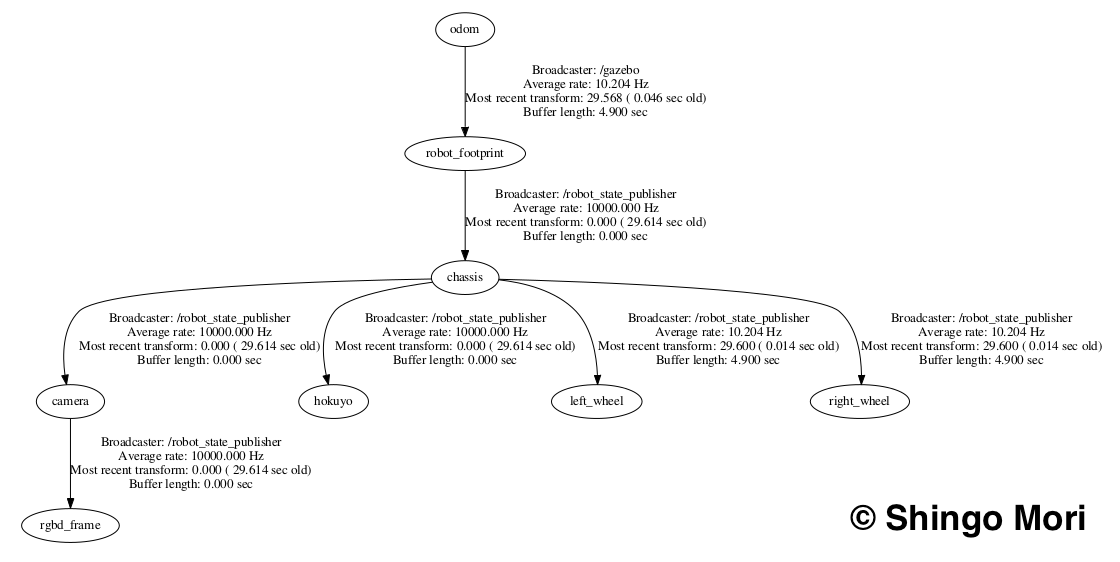
\includegraphics[width=0.64\linewidth]{tf_view}\label{fig:tf-view}}
      \caption{Robot model setup.}
\end{figure}

Sensor parameters for the RGB-D camera and laser range finder is set based on published specification of Kinect v1 and Hokuyo, respectively.

\subsection{Packages Used}
Two official ROS packages are used for this project. The rtabmap package is used for solving the SLAM problem, and the teleop package is used to manally navigating the robot. 

\subsubsection{Parameters}
All the parameters related to the algorithm are supplied by Udacity and used as is.

\section{Results}
The estimated pose and map for the Kitchen Dining environment is shown in Fig. \ref{fig:result-supplied}. The robot travelled for approximately 106 meters, and 27 loop closures were detected along the path.

\begin{figure}[thpb]
      \centering
      \subfloat[2D grid Map. Black dots represent the occupied grid, blue lines represent the robot path, and red lines represent the detected loop closures.]{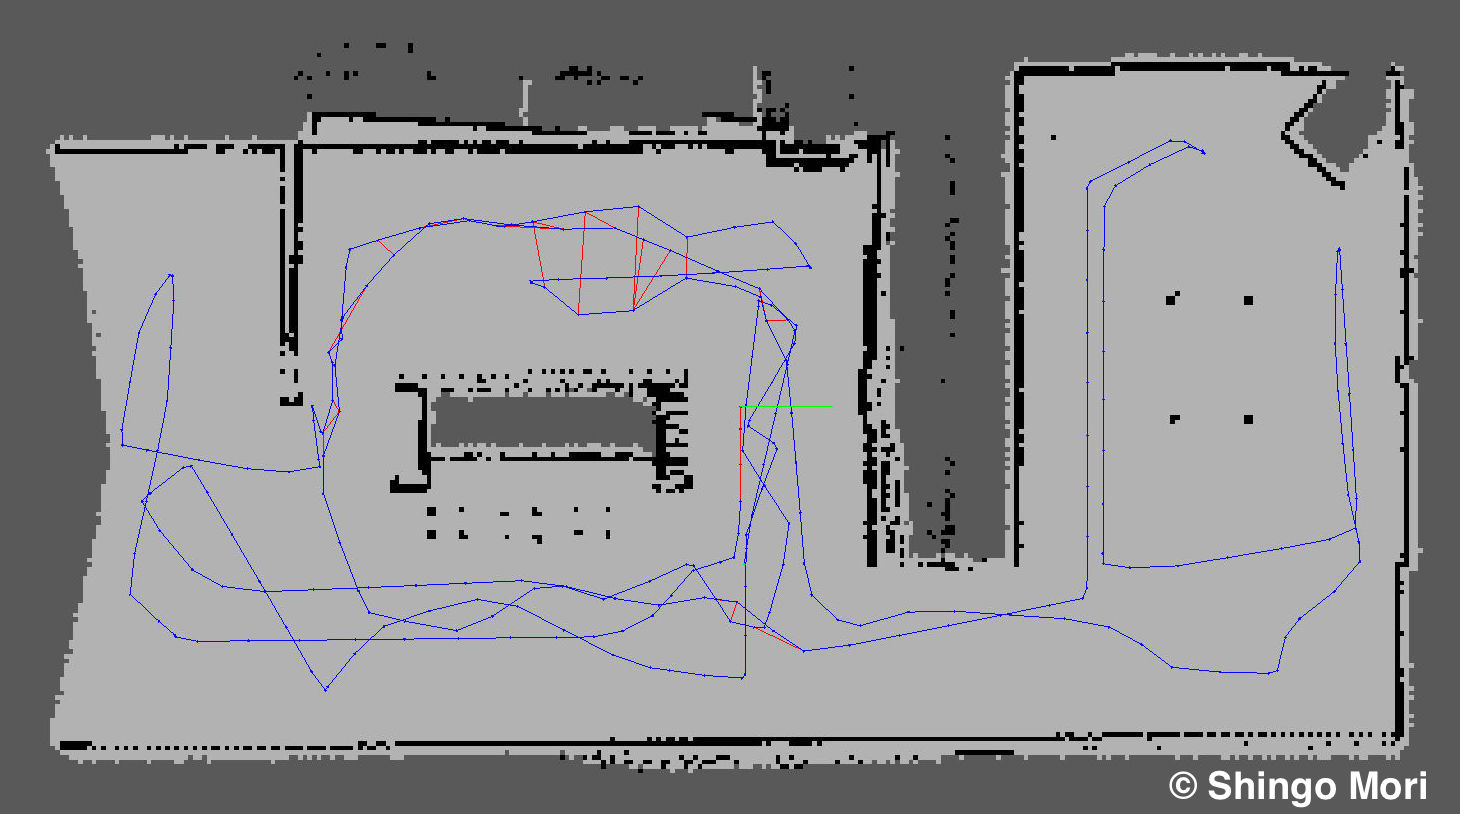
\includegraphics[width=0.95\linewidth]{result-supplied-2d}}
      \vfill
      \subfloat[3D point cloud.]{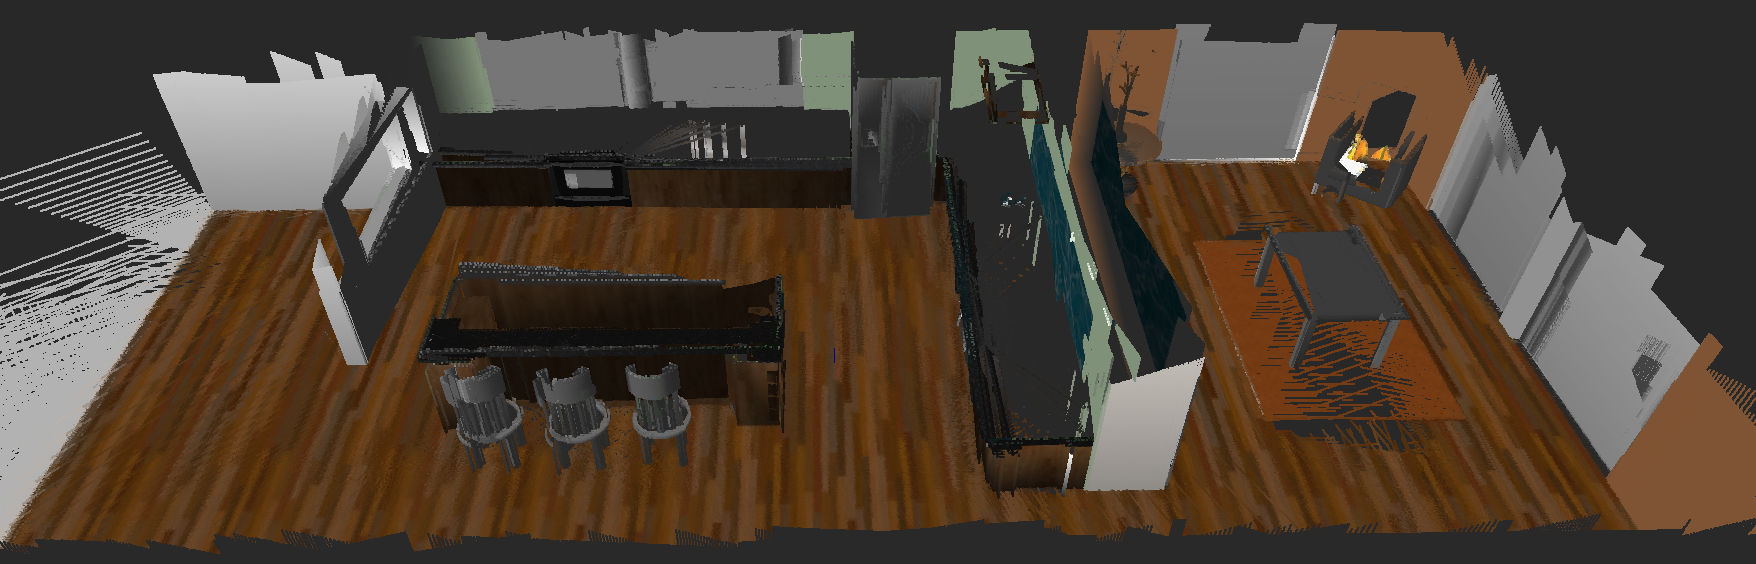
\includegraphics[width=0.95\linewidth]{result-supplied-3d}}
      \caption{Generated maps for the Kitchen Dining environment.}
      \label{fig:result-supplied}
\end{figure}

The estimated pose and map for the Bot Cafe environment is shown in Fig. \ref{fig:result-personal}. The robot travelled for approximately 79 meters, and 2 loop closures were detected on along the path. There are some noticeable errors in the generated 2D map such as duplicate wall-points.

\begin{figure}[thpb]
      \centering
      \subfloat[2D grid Map. Black dots represent the occupied grid, blue lines represent the robot path, and red lines represent the detected loop closures.]{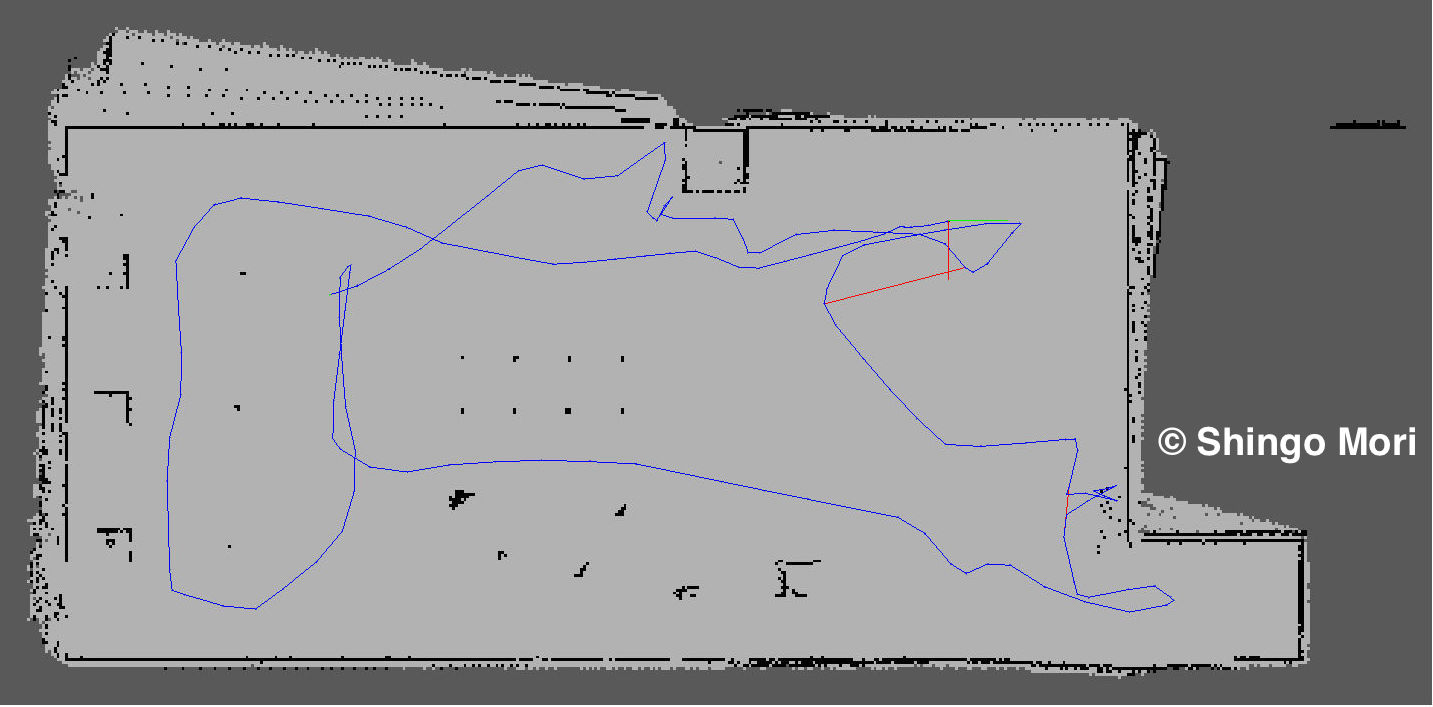
\includegraphics[width=0.95\linewidth]{result-personal-2d}}
      \vfill
      \subfloat[3D point cloud.]{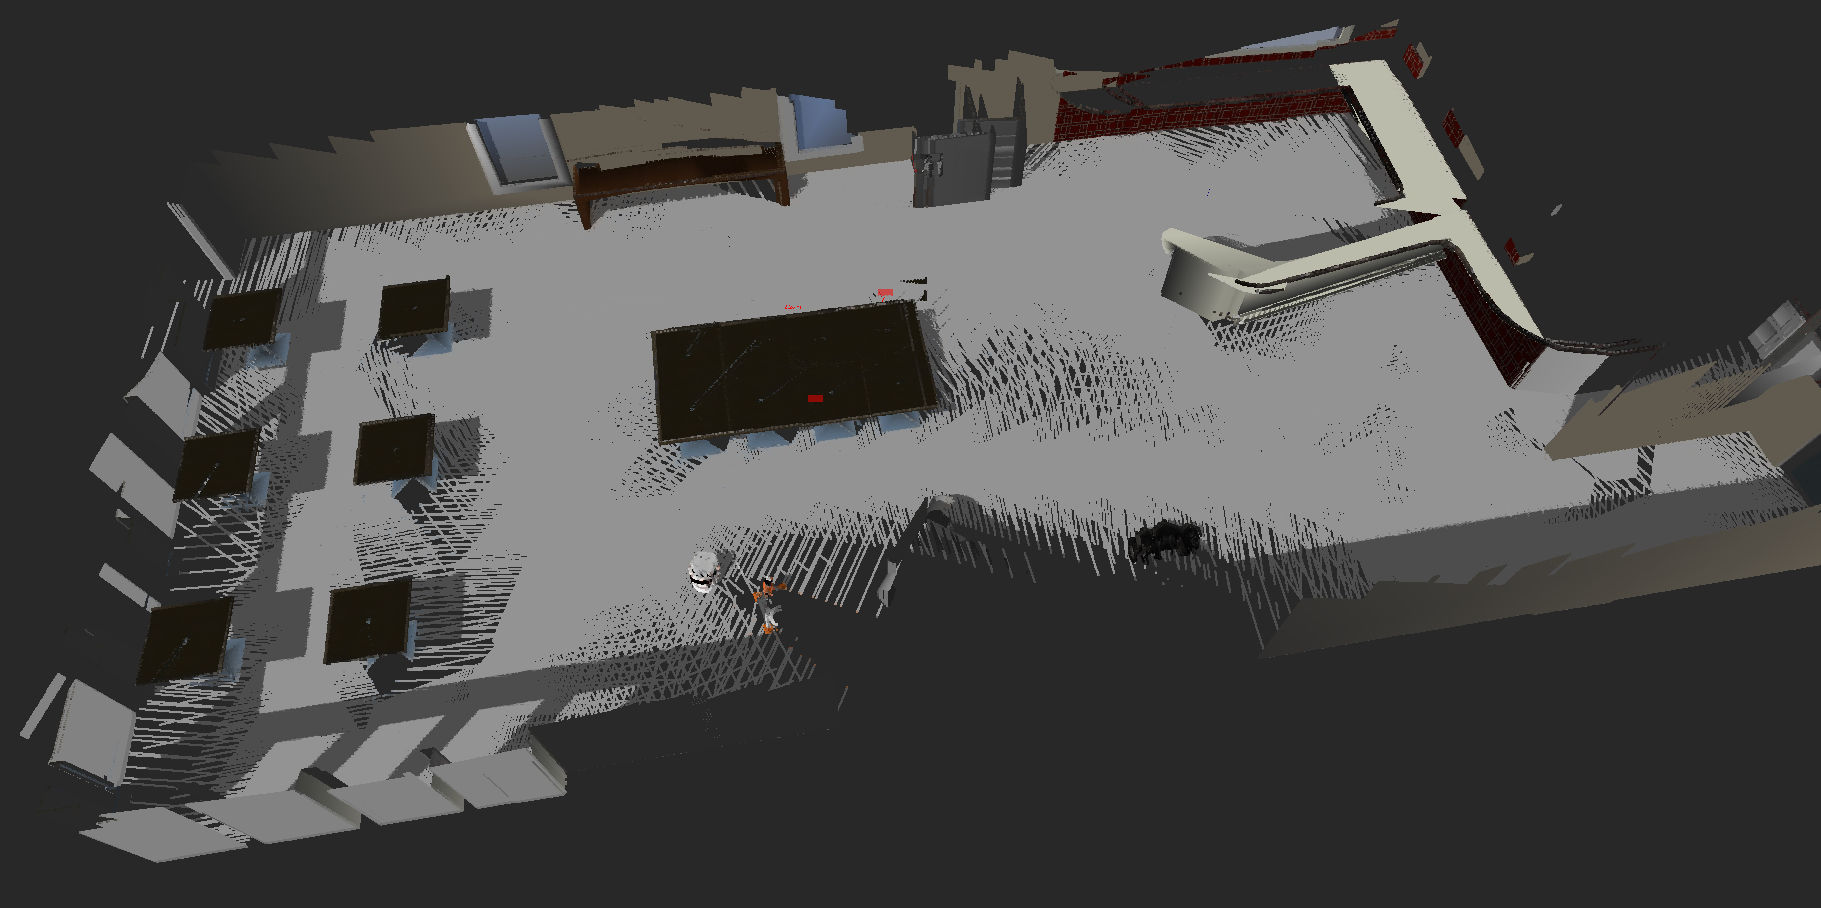
\includegraphics[width=0.95\linewidth]{result-personal-3d}}
      \caption{Generated maps for the Bot Cafe environment.}
      \label{fig:result-personal}
\end{figure}

\section{Discussion}
The quality of the generated 2D map is higher for the Kitchen Dining than the one for the Bot Cafe. This is probably due to the difference in the number of loop closures detected. In the Bot Cafe environment where many open areas exist inside, only a few number of loop closures (2) are detected. In contrast, more than 10 times the number of loop closures (27) are detected in the Kitchen Dining environment, where the robot is almost always surrounded by distinct features. Less number of detected loop closures in the Bot Cafe caused it difficult for the SLAM algorithm to reduce the error during its optimization process, resulting in the less accurate pose estimation and map generation.

Although there are some errors exist in the generated maps, the amount of cumulative error is limited and the overall accuracy is acceptable for the both environments. If a global-localization algorithm is applied, it should be able to localize the robot accurately using the estimated 2D map in each environment.

\section{Conclusion / Future work}
A ROS package is created and RTAB-Map is utilized to solve the SLAM problem in a gazebo environment. A robot is manually controlled in the environment, and 2D/3D maps are created in real-time using the sensor data acquired by the robot. The package is tested in two different scenes, and the algorithm works well in the both environment.

The quality of the estimated map is highly dependent on the number of loop closures detected. More robust feature detection technique are needed to deal with open-areas.

Although the parameters of the sensors are properly set, their noises are still limited in the simulated environment. For the future work, the performance of the package will be tested in the real environment. 

\bibliography{bib}
\bibliographystyle{ieeetr}

\end{document}